\documentclass[times,specification,annotation]{itmo-student-thesis}

%% Опции пакета:
%% - specification - если есть, генерируется задание, иначе не генерируется
%% - annotation - если есть, генерируется аннотация, иначе не генерируется
%% - times - делает все шрифтом Times New Roman, собирается с помощью xelatex
%% - languages={...} - устанавливает перечень используемых языков. По умолчанию это {english,russian}.
%%                     Последний из языков определяет текст основного документа.

%% Делает запятую в формулах более интеллектуальной, например:
%% $1,5x$ будет читаться как полтора икса, а не один запятая пять иксов.
%% Однако если написать $1, 5x$, то все будет как прежде.
\usepackage{icomma}

%% Один из пакетов, позволяющий делать таблицы на всю ширину текста.
\usepackage{tabularx}

%% Данные пакеты необязательны к использованию в бакалаврских/магистерских
%% Они нужны для иллюстративных целей
%% Начало
\usepackage{tikz}
\usetikzlibrary{arrows}
\usepackage{filecontents}



\DeclareMathOperator*{\argmax}{argmax}
\DeclareMathOperator*{\argmin}{argmin}

\begin{filecontents}{bachelor-thesis.bib}
@online{ doerr-doerr-lambda-lambda-self-adjustment-arxiv,
    year        = {2020},
    title       = {Optimal Parameter Choices Through Self-Adjustment: Applying the 1/5-th Rule in
                   Discrete Settings},
    author      = {Benjamin Doerr and Carola Doerr},
    url         = {http://arxiv.org/abs/1504.03212},
    year        = {2015},
    langid      = {english}
}

% @inproceedings{ example-english,
%     year        = {2015},
%     booktitle   = {Proceedings of IEEE Congress on Evolutionary Computation},
%     author      = {Maxim Buzdalov and Anatoly Shalyto},
%     title       = {Hard Test Generation for Augmenting Path Maximum Flow 
%                    Algorithms using Genetic Algorithms: Revisited},
%     pages       = {2121-2128},
%     langid      = {english}
% }

@article{ example-russian,
    author      = {Тельнов Сергей Андреевич},
    title       = {Моделирование ставок в аукционе},
    number      = {2(72)},
    year        = {2011},
    pages       = {72-77},
    langid      = {russian}
}

% @article{ unrestricted-jump-evco,
%     author      = {Maxim Buzdalov and Benjamin Doerr and Mikhail Kever},
%     title       = {The Unrestricted Black-Box Complexity of Jump Functions},
%     journal     = {Evolutionary Computation},
%     year        = {2016},
%     note        = {Accepted for publication},
%     langid      = {english}
% }

% @book{ bellman,
%     author      = {R. E. Bellman},
%     title       = {Dynamic Programming},
%     address     = {Princeton, NJ},
%     publisher   = {Princeton University Press},
%     numpages    = {342},
%     pagetotal   = {342},
%     year        = {1957},
%     langid      = {english}
% }
\end{filecontents}
%% Конец

%% Указываем файл с библиографией.
\addbibresource{bachelor-thesis.bib}

\begin{document}

\studygroup{M3435}
\title{Моделирование ставок в аукционе}
\author{Тельнов Сергей Андреевич}{Тельнов С.А.}
\supervisor{Фильченков Андрей Александрович}{Фильченков А.А.}{к.ф.-м.н., доцент ФИТиП}{Университета ИТМО}
\publishyear{2020}
%% Дата выдачи задания. Можно не указывать, тогда надо будет заполнить от руки.
\startdate{01}{сентября}{2020}
%% Срок сдачи студентом работы. Можно не указывать, тогда надо будет заполнить от руки.
\finishdate{31}{мая}{2020}
%% Дата защиты. Можно не указывать, тогда надо будет заполнить от руки.
\defencedate{15}{июня}{2020}

\addconsultant{Яковлева Д.В.}{магистр}

\secretary{Павлова О.Н.}

%% Задание
%%% Техническое задание и исходные данные к работе
\technicalspec{Требуется че-то там, чтобы получить че-то там.}

%%% Содержание выпускной квалификационной работы (перечень подлежащих разработке вопросов)
\plannedcontents{Сделал че-то там, получил че-то там.}

%%% Исходные материалы и пособия 
\plannedsources{\begin{enumerate}
    \item ГОСТ~7.0.11-2011 <<Диссертация и автореферат диссертации>>;
    \item С.М. Львовский. Набор и верстка в системе \LaTeX;
    \item предыдущий комплект стилевых файлов, использовавшийся на кафедре компьютерных технологий.
\end{enumerate}}

%%% Цель исследования
\researchaim{Разработка удобного стилевого файла \LaTeX
             для бакалавров и магистров кафедры компьютерных технологий.}

%%% Задачи, решаемые в ВКР
\researchtargets{\begin{enumerate}
    \item обеспечение соответствия титульной страницы, задания и аннотации шаблонам, принятым в настоящее время на кафедре;
    \item обеспечение соответствия содержательной части пояснительной записки требованиям ГОСТ~7.0.11-2011 <<Диссертация и автореферат диссертации>>;
    \item обеспечение относительного удобства в использовании~--- указание данных об авторе и научном руководителе один раз и в одном месте, автоматический подсчет числа тех или иных источников.
\end{enumerate}}

%%% Использование современных пакетов компьютерных программ и технологий
% \addadvancedsoftware{Пакет \texttt{tabularx} для чуть более продвинутых таблиц}{\ref{sec:tables}, Приложения~\ref{sec:app:1}, \ref{sec:app:2}}
% \addadvancedsoftware{Пакет \texttt{biblatex} и программное средство \texttt{biber}}{Список использованных источников}

%%% Краткая характеристика полученных результатов 
\researchsummary{Получился, надо сказать, практически неплохой стилевик. В 2015--2018 годах
его уже использовали некоторые бакалавры и магистры. Надеюсь на продолжение.}

%%% Гранты, полученные при выполнении работы 
\researchfunding{Автор разрабатывал этот стилевик исключительно за свой счет и на
добровольных началах. Однако значительная его часть была бы невозможна, если бы
автор не написал в свое время кандидатскую диссертацию в \LaTeX,
а также не отвечал за формирование кучи научно-технических отчетов по гранту,
известному как <<5-в-100>>, что происходило при государственной финансовой поддержке
ведущих университетов Российской Федерации (субсидия 074-U01).}

%%% Наличие публикаций и выступлений на конференциях по теме выпускной работы
\researchpublications{По теме этой работы я (к счастью!) ничего не публиковал.
    \begin{refsection}
        Однако покажу, как можно ссылаться на свои публикации из списка литературы:
    \nocite{example-english, example-russian}
    \printannobibliography
    \end{refsection}
}

%% Эта команда генерирует титульный лист и аннотацию.
\maketitle{Бакалавр}

%% Оглавление
\tableofcontents

%% Макрос для введения. Совместим со старым стилевиком.
\startprefacepage

Аукцион в реальном времени (англ. RTB) появился в 2009 году и 
стал одним из самых важных механизмов в онлайн-рекламе.
Рекламодатели начали платить за каждый аукцион отдельно, основываясь на своих стратегий торгов. 
От качества выбранной стратегии напрямую зависит эффективность рекламы.

Ежедневно в сети проходит огромное количество аукционов 
и проследить стратегию каждого отдельного игрока не представляется возможным.
Поэтому можно подстроить алгоритм, который будет предсказывать количество выигранных аукционов для каждой ставки.
Основываясь на этой статистике, рекламодатели или рекламные агентства смогут 
построить свою стратегию ведения торгов для повышения показателей эффективности каждого рекламного объявления.


%% Начало содержательной части.
\chapter{Описание и анализ предметной области}

Введем основные понятия и определения из предметной области, которые необходимы для описания постановленной задачи.

\section{Онлайн-реклама}

\begin{definition}
    Онлайн-реклама – это форма маркетинга, которая использует интернет,
    чтобы доставить маркетинговое сообщения до потенциального покупателя.
    \footnote{https://en.wikipedia.org/wiki/Online_advertising}
\end{definition}

Онлайн-рекламу можно увидеть на большинстве интернет-страницах в виде баннера.
Контекст и тематика рекламы чаще всего совпадает со сферой интересов посетителей сайта,
для увеличения показателей эффективности объявления.

\begin{figure}[h]
    \label{fig:banner}
    \caption{Пример рекламного баннера на сайте rbc.ru}
    \centering
    
\includegraphics{banner-example.png}
\end{figure}

\section{Онлайн-реклама}

\begin{definition}
    Онлайн-аукцион – процесс выбора рекламного объявления для показа пользователю.
    Кандидаты на показ предлагают свою ставку и выигрывает участник с наибольшей ценой.
    \footnote{\label{fn:auction}https://ru.wikipedia.org/wiki/Аукцион}
\end{definition}

Аукционы могут быть открытыми или закрытыми.
В закрытом аукционе участники не видят ставку своих оппонентов и не могут изменять свои ставки,
в отличии от открытого аукциона, где все участники видят ставки друг друга.

\begin{definition}
    Аукцион первой цены – закрытый аукцион, при котором победителем является участник
    с самой высокой ценой и именно эта цена подлежит уплате.
    \footnoteref{fn:auction}
    \footnoteref{fig:banner}
\end{definition}

\begin{definition}
    Аукцион второй цены – закрытый аукцион, при котором победителем является участник с самой высокой ценой,
    но уплатить он должен <<вторую цену>>, то есть цену своего ближайшего конкурента.
    \footnote{\label{fn:auction}https://ru.wikipedia.org/wiki/Аукцион}.
\end{definition}

% \footnote{http://www.adnews.com.au/opinion/how-to-better-understand-auction-dynamics-for-video-ad-campaigns}
\begin{figure}[h]
    \label{fig:auction}
    \caption{Пример аукциона второй и первой цены}
    \centering
    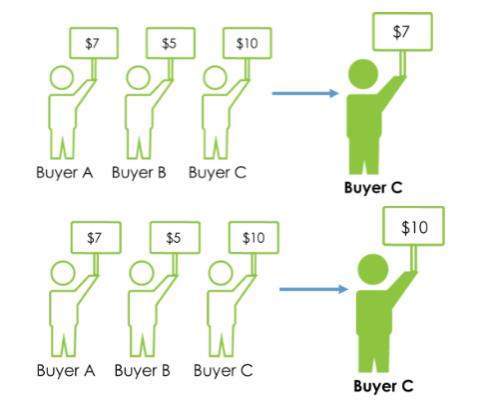
\includegraphics{s_f_price-auction.png}
\end{figure}

\begin{definition}
    Рыночная цена – цена, которую платит победитель аукциона.
\end{definition}

\begin{definition}
    RTB (Real Time Bidding) – технология закупки медийной рекламы посредством программируемых онлайн-аукционов
    \footnote{\label{fn:rtb} http://rtb-media.ru/wiki/}.
\end{definition}

RTB фокусируется непосредственно на показах целевым посетителям,
а не планированию резервов рекламных площадей на определенных сайтах. 
Каждый показ выкупается за доли секунды – во время загрузки страницы – система. 
RTB мгновенно проводит аукцион. В результате лучшее предложение от рекламодателей появляется на глазах пользователя, которому оно наиболее интересно. 

\begin{figure}[h]
    \caption{Механика работы RTB}
    \centering
    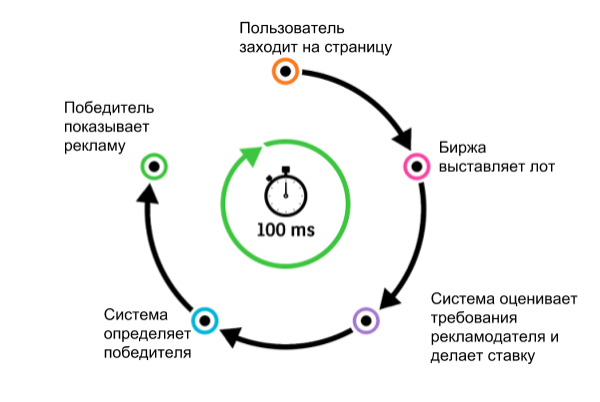
\includegraphics{rtb-example.png}
\end{figure}

Ставка в аукционе основывается на информации о пользователе, 
который заходит на веб-страницу, 
и потенциальной выгоде, которую он может принести.

О пользователе рекламодатели знают информацию 
о дате и времени захода на сайт, регион, URL сайта, где будет выставлена реклама, 
размер рекламного баннера и интересы пользователя (таргеринг). 
Далее эту информацию будем называть как запрос для ставки.

Выгода от рекламного объявления является позитивным ответом пользователя, показатели CTR и CVR.

\begin{definition}
    CTR (Click-through rate) – метрика в интернет-маркетинге, 
    которая определяется как отношение числа кликов на рекламное объявление к числу показов.
    \footnote{https://ru.wikipedia.org/wiki/CTR_(Интернет)}
\end{definition}

\begin{definition}
    Конверия (англ. Conversion rate) – это отношение числа посетителей сайта, выполнивших на нём какие-либо целевые действия.
    \footnote{https://ru.wikipedia.org/wiki/Конверсия_(в_интернет-маркетинге)}
\end{definition}


\section{Машинное обучение}

\begin{definition}
    Машинное обучение – подраздел искусственного интеллекта, изучающий обучающиеся методы построения алгоритмов.
    \footnote{\label{fn:ml_neerc} https://neerc.ifmo.ru/wiki/index.php?title=Общие_понятия#.D0.9E.D0.B1.D1.83.D1.87.D0.B5.D0.BD.D0.B8.D0.B5_.D0.B1.D0.B5.D0.B7_.D1.83.D1.87.D0.B8.D1.82.D0.B5.D0.BB.D1.8F_.28.D0.B0.D0.BD.D0.B3.D0.BB._Unsupervised_learning.29}
\end{definition}

\begin{definition}
    Компьютерная '''программа обучается''' на основе опыта $E$ по отношению к некоторому классу задач $T$ и меры качества $P$,
    если качество решения задач из $T$, измеренное на основе $P$, улучшается с приобретением опыта $E$.
    \footnotemark[\ref{fn:ml_neerc}]
\end{definition}

\begin{definition}
    Обучение с учителем (англ. Supervised learning) – один из способов машинного обучения, 
    в ходе которого испытуемая система обучается с помощью пары <<объект, ответ>>.
    Цель обучения в восстановлении зависимости между множеством <<объектов>> и <<ответов>>.
\end{definition}

\begin{definition}
    Обучение без учителя (англ. Unsupervised learning) изучает широкий класс задач обработки данных, 
    в которых известны только описания множества объектов (обучающей выборки), и 
    требуется обнаружить внутренние взаимосвязи, зависимости, закономерности, существующие между объектами.
    \footnote{http://www.machinelearning.ru/wiki/index.php?title=Обучение_без_учителя}
\end{definition}

\begin{definition}
    Кластерный анализ (англ. Data clustering) — задача разбиения заданной выборки объектов (ситуаций) на непересекающиеся подмножества, 
    называемые кластерами, так, чтобы каждый кластер состоял из схожих объектов, а объекты разных кластеров существенно отличались.
    \footnote{http://www.machinelearning.ru/wiki/index.php?title=Кластеризация}
\end{definition}

\begin{definition}
    Искусственные нейронная сеть (англ. artificial neural network; ANN) — это математическая модель, а также ее программные или аппаратные реализации,
    построенная в некотором смысле по образу и подобию сетей нервных клеток живого организма.
    \footnote{http://www.machinelearning.ru/wiki/index.php?title=Искусственная_нейронная_сеть}
\end{definition}

\begin{definition}
    Рекуррентные нейронные сети (англ. Recurrent neural network; RNN) — вид нейронных сетей, 
    где связи между элементами образуют направленную последовательность. 
    Благодаря этому появляется возможность обрабатывать серии событий во времени или последовательные пространственные цепочки.
    \footnote{https://ru.wikipedia.org/wiki/Рекуррентная_нейронная_сеть}
\end{definition}

\section{Survival Analysis}

\begin{definition}
    Survival analysis – это класс статических моделей, позволяющий оценить вероятность наступления событий.
\end{definition}

Цель анализа в оценке времени, когда произойдет интересующее событие.

\begin{definition}
    Функция выживания (англ. Survival Function) определяет вероятность того, что интересующее событие не произойдет в момент времени \(t\).
\end{definition}

\begin{equation}\label{eq:sa}
    S(t) = Pr(T > t) = \int\limits_{t}^{\infty} f(u) du
\end{equation}

Функция $f(x)$ – плотность распределения вероятности наступления события в момент времени $x$.
В Survival analysis называется, как <<rate of death>> или <<failure events per unit time>>.

Функция условной вероятности определяет, что событие произойдет в рассматриваемый интервал времени, 
при условии, что оно не произошло до этого интервала.

\begin{equation}
    h(t) = \lim_{\delta t\to\infty} \frac{Pr(t \leq T \leq t + \delta t \mid T > t)}{\delta t}
\end{equation}

\begin{definition}
    Оценка Каплана-Мейера – непараметрическая функция, используется для оценки Функции выживания~\ref{eq:sa}
\end{definition}

\begin{equation}\label{eq:rm}
    \hat{S}(t) = \prod_{i: t_i \leq t} (1 - \frac{d_i}{n_i})
\end{equation}

\section{Постановка задачи}

Цель данной работы улучшить предсказание плотности распределения рыночной цены в аукционе второй цены.

\begin{figure}[h]\label{fig:problem}
    \caption{Задача предсказания ставок в аукционе}
    \centering
    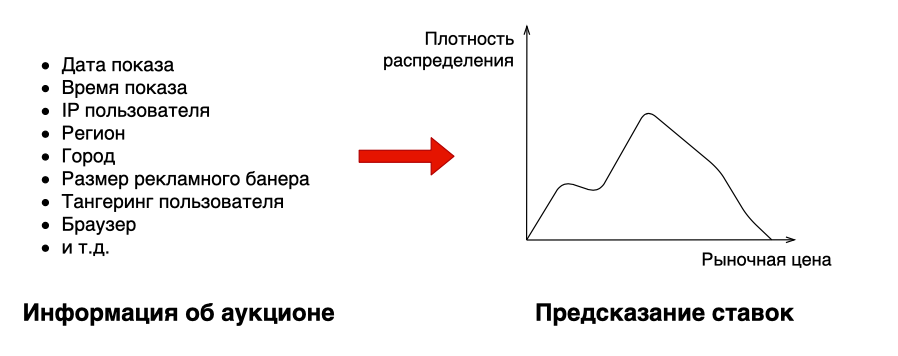
\includegraphics{problem.png}
\end{figure}

Более формально. По запросу (информации о пользователе) $x$ получить распределение рыночной цены $p(x)$.

Для решения будет использоваться истории ставок в аукционе, 
каждый пример можно представить как тройку значений $(x, z, b)$, 
где $x$ – информация о пользователе, 
$z$ – рыночная цена аукциона, 
$b$ – ставка рекламодателя.

Аукцион закрытый, поэтому рыночная цена известна, только если рекламодатель выиграет аукцион. То есть в случае $b > z$.

С помощью плотности распределения можно будет рассчитывать вероятность выигрыша и проигрыша аукциона для любой интересующей ставки.

Будем решать сведением задачи к Survival analysis и использованием глубоких нейронных сетей.

\chapterconclusion

В данной главе были определены основные понятия и определения об онлайн-рекламе и онлайн-аукционе, 
рассмотрена задача Survival analysis и поставлена задача.


\chapter{Теоретическое исследование}

В первой главы были введены основные определения и сформулирована задача данной работы. 
В этой главе будут рассмотрены существующие решения этой задачи и новые подходы для улучшения существующих результатов.

\section{Анализ существующих решений}

В этом разделе будут описаны решения задачи предсказания ставок в аукционе, 
с помощью сведения к Survival Analysis и без использования нейронных сетей.

\subsection{Аналитическое решение}

Рассмотрим статью 2016 года, которая была опубликована авторами Weinan Zhang, Tianxiong Zhou, Jun Wang, Jian Xu. 
В этой статье не использовалась информация о пользователе, а учитывалась только ставка рекламодателя и рыночная цена аукциона.

В этой статье решили задачу нахождения вероятности проигрыша/выигрыша аукциона с заданной ставкой с помощью сведения к Survival analysis.

Переведем тройку значений $(b_i, w_i, z_i )_{i=1..N}$, где $b_i$ – ставка, $z_i$ – рыночная цена, $w_i$ – выигрыш/проигрыш аукциона, 
в формат $(b_j,d_j,n_j )_{j=1..M}$. Где $d_j$ – число выигранных аукционов с рыночной ценой равной 
$b_{j-1}$ (по аналогии, интересующее нам событие происходит в день $b_j$). 
$n_j$ – число аукционов, которые не могут быть выиграны со ставкой $b_j$, 
то есть число выигранных аукционов с рыночной ценой не менее $b_{j-1}$ и число проигранных, 
в которых ставка была не менее $b_{j-1}$. А саму ставку $b_j$ можно рассматривать как $b_j$ день наблюдения.

Тогда вероятность проигрыша аукциона со ставкой $b_x$, используя формулу ~\ref{eq:rm}, будет равна:

\begin{equation}
    s(b_x) = \prod_{b_j < b_x} \frac{n_j - d_j}{n_j}
\end{equation}

Что в Survival Analysis аналогично вероятности того, что интересующее событие не произойдет в интервале от $1$ до $b_x$.

Вероятность выигрыша будет равна:

\begin{equation}
    w(b_x) = 1 - s(b_x) = 1 - \prod_{b_j < b_x} \frac{n_j - d_j}{n_j}
\end{equation}

Плотность распределения рыночной цены:

\begin{equation}
    p(z)=w(z+1)-w(z)=s(z)-s(z+1)
\end{equation}

\subsection{Решение с использованием решающих деревьев}

Большой недостаток решения, описанного в прошлом разделе, в том, что не используется информация о пользователе. 
В статье, опубликованной в 2016 году, для это была использована задача кластеризации.
Для получения распределение рыночной цены $p_x (z)$ используется бинарное дерево решений $T_p (x)$. 
Главная идея в кластеризации данных, используя информацию о пользователях. 
Для этого используется метод k-средних и расстояние Кульбака-Лейблера $D_{KL}$.

Дивергенция Кульбака-Лейблера $D_{KL} (q \mid p)$ является мерой расстояния между двумя вероятностными распределениями $q(x)$ и $p(x)$

\begin{equation}
    D_{KL} = - \int q(x) \log \frac{p(x)}{q(x)} dx
\end{equation}

При построении дерева в каждом узле будет выбираться разбиение с максимальным расстоянием Кульбака-Лейблера $D_{KL}$. 
Математически алгоритм разбиения будет выглядеть следующим образом.

\begin{equation}
    \begin{split}
        T_p^{\pi} (x) & = \argmax_{\pi} \sum_{i = 1}^l D_{KL}^i \\
        D_{KL}^i & = max {D_{KL}^{i1}, D_{KL}^{i2}, ..., D_{KL}^{ij}, ..., D_{KL}^{iN}} \\
        D_{KL}^{ij} & = \sum_{z = 1}^{z_{max}} p_x(z) \log \frac{p_x(z)}{q_x(z)}
    \end{split}
\end{equation}

Где $p$ и $q$ – это вероятность распределения разбиения, 
$z_max$ – наибольшая рыночная цена, 
$D_{KL}^{ij}$ – наибольшее расстояние Кульбака-Лейблера среди всех признаков $A_j$ в $i$-ом узле,
$N=  |\Theta|$ - количество признаков,
$l$ – количество разбиений.

Тогда для предсказание будет выбираться кластер, проходом по дереву, и в листе считаться $p_x (z)$.
Сама плотность распределения считается аналогично статье (номер статьи), 
также задача сводиться к Survival analysis, только статистические данные считаются для каждого кластера отдельно.

\section{Решение с использованием глубокого обучения}

Главная цель этой работы состоит в улучшении показателей решения, которого будет описано в этом разделе.
В 2019 году студенты Китайского университета Шанхая опубликовали статью про использование глубоких рекуррентных нейронных сетей в Survival Analysis, 
и также сделали отдельную публикацию использования этого решения в предсказании рыночной цены в аукционах.

В первой статье были опубликованы показатели применения нового решения в разных областях: 
в медицине, музыкальной индустрии и предсказании ставок в аукционе. 
По результатам эксперимента это решение выдала лучшие показатели ROC-кривой (как бинарного классификатора) и 
ANLP (average negative log probability) среди всех известных на тот момент решений.

Это решение взято за baseline и именно его мы будем пытаться улучшить.

\subsection{Сведение Survival Analysis к задаче предсказания ставок}

Во второй статье было описано как задачу Survival Analysis свели к нахождению распределения вероятности рыночной цены 
и поставленную задачу решили с помощью глубоких нейронных сетей.

Для введения вероятностей выигрыша и проигрыша в аукционе 
с заданной ставкой была использована формула ~\ref{eq:sa}.

\begin{figure}[h]
    \caption{Плотность распределения в непрерывном пространстве}
    \centering
    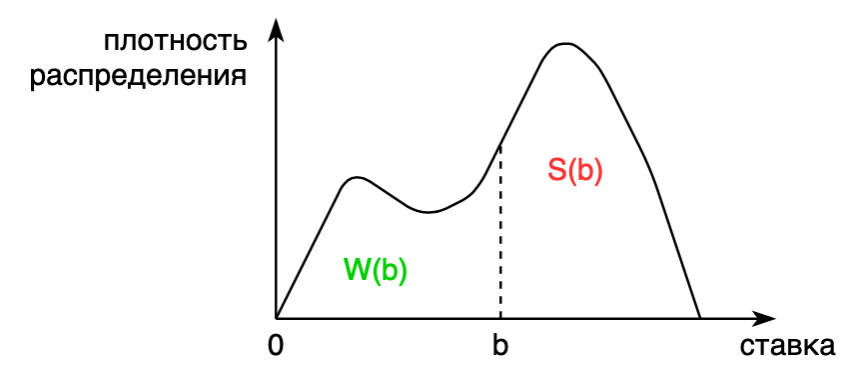
\includegraphics{w_s_curve.png}
\end{figure}

\begin{equation}
    \begin{split}
        W(b) & = Pr(z < b) = \int\limits_{0}^b p(x) dx \\
        S(b) & = Pr(z \geq b) = 1 - W(b) = \int\limits_{b}^{\infty} p(x) dx \\
        p(b) & = W(b + 1) - W(b) = S(b) - S(b + 1)            
    \end{split}
\end{equation}

Чтобы нейронная сеть смогла обучаться предсказывать плотность распределения, 
необходимо перейти из непрерывного пространства в дискретное.
Для этого представим ставки как последовательность 
от наименьшей до наибольшей $0<b_1<b_2< ...< b_L$ и выберем $L$ блоков $V_l$ таких, 
что для $l=1, 2, …, L$ блок $V_l=(b_l,b_{l+1}]$.

\begin{figure}[h]
    \caption{Плотность распределения в дискретном пространстве}
    \centering
    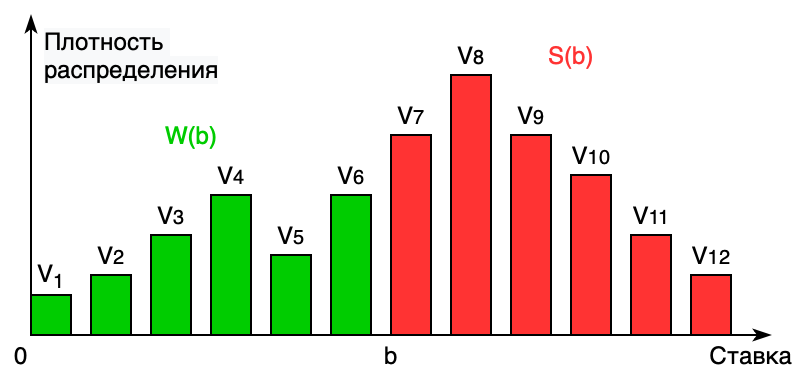
\includegraphics{w_s_discret.png}
\end{figure}

Все ставки принадлежал множеству натуральных чисел и для лучшего предсказания $\forall l$  $b_{l+1}-b_l=1$.

Тогда формулы вероятностей будут иметь следующий вид.

\begin{equation}
    \begin{split}
        W(b_l) & = Pr(z < b_l) = \sum_{j<l} Pr(z \in V_j) \\
        S(b_l) & = Pr(z \geq b_l) = \sum_{j \geq l} Pr(z \in V_j) \\
        p(b_l) & = Pr(z \in V_l) =  W(b_{l + 1}) - W(b_l) = S(b_l) - S(b_{l + 1})
    \end{split}
\end{equation}

Введем формулу условной вероятности выигрыша в аукционе для ставки $b_l$. 
Это значение будет предсказывать нейронная сеть.

\begin{equation}
    h_l = Pr(z \in V_l \mid z \geq b_{l - 1}) = \frac{Pr(z \in V_l)}{Pr(z \geq b_{l - 1})} = \frac{p_l}{S(b_{l - 1})}
\end{equation}

\subsection{Описание работы нейронной сети}

Для предсказания условной вероятности используется 
$f_{\Theta}$ – функция рекуррентной нейронной сети, 
которая приминается пару значений $(x, b_l)$, 
где $x$ – информация о пользователе, а $b_l$ – ставка.

В выходе нейронной сети $L$ блоков – условная вероятность выигрыша аукциона для пользователя с информацией $x$ и ставкой $b_l$. 
Используя значения об условной вероятности, можно найти вероятности выигрыша, проигрыша и плотность распределения рыночной цены.

Формула условной вероятности для $x^i$ и блока $l$. $r_{l-1}$ – скрытый вектор из предыдущего рекуррентного блока.

\begin{equation}
    h_l^i = Pr⁡(z \in V_l \mid z \geq b_{l-1}, x^i; \Theta)= f_{\Theta} (x^i, b_l \mid r_{l-1})
\end{equation}

Вероятность проигрыша и выигрыша в аукционе для примера $x^i$, со ставкой $b_l$ будет равны:

\begin{equation}\label{eq:nnS}
    \begin{split}
        S(b_l \mid x^i; \Theta) & = Pr(z \geq b_l \mid x^i; \Theta) = Pr(z \notin V_1, z \notin V_2, ..., z \notin V_l \mid x^i; \Theta) \\
        & = Pr(z \notin V_1 \mid x^i; \Theta) \cdot Pr(z \notin V_2 \mid z \notin V_1, x^i; \Theta) ... \\
        & \cdot Pr(z \notin V_l \mid z \notin V_1, ..., z \notin V_{l - 1},  x^i; \Theta) \\
        & = \prod_{l_j : l_j \leq l} \left[1 - Pr(z \in V_{l_j} \mid z \geq b_{l_j}, x^i; \Theta)\right] = \prod_{l_j: l_j \leq l} (1 - h_{l_j}^i)
    \end{split}
\end{equation}

\begin{equation}\label{eq:nnW}
    W(b_l \mid x^i; \Theta) = Pr(b_l > z \mid x^i; \Theta) = 1 - S(b_l \mid x^i; \Theta) = 1 - \prod_{l_i: l_i \leq l} (1 - h_l^i)
\end{equation}

И плотность распределения рыночной цены будет равна:

\begin{equation}\label{eq:nnP}
    p_l^i = Pr(z^i \in V_l \mid x^i; \Theta) = h_{l^i}^i \prod_{l: l < l^i} (1 - h_l^i)
\end{equation}


\section{Описание решения}

В данном разделе будет описания решения, которое реализовано на данный момент, устройство нейронной сети, обучение и метрики для проверки качества.

\subsection{Устройство нейронной сети}

\begin{figure}[h]
    \caption{Иллюстрация нейронной сети}
    \centering
    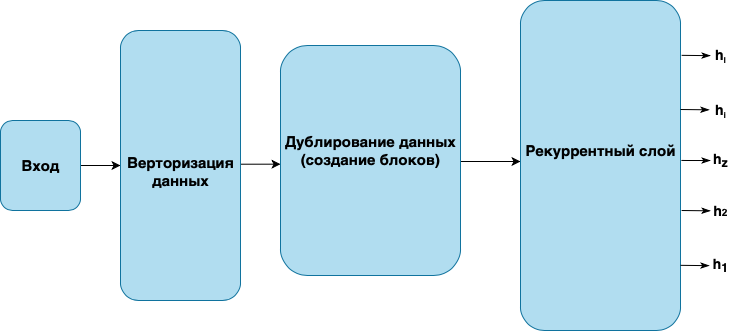
\includegraphics{nn.png}
\end{figure}

Для наглядности разобьем нашу нейронную сеть на три части.

В первой части модели происходит перевод переданных примеров в формат, необходимый для вычисления. 
Этот процесс выполняют первые два слоя: Embedding переводит слова в векторное представление, 
Dense слой уменьшает размерность примеров, для увеличения производительности.

Во второй части переводим данных в формат, который будет удобен для предсказания ставки. 
Переданные данные дублируются ровно столько раз, сколько мы хотим предсказать условных вероятностей. 
То есть в этом слое создаются блоки ставок, которые были описаны выше в разделе 2.2.2.
После дублирования к каждому блоку добавляется еще один параметр – номер блока, который является значением ставки в этом блоке.


\begin{figure}[h]
    \caption{Иллюстрация работы рекуррентного слоя}
    \centering
    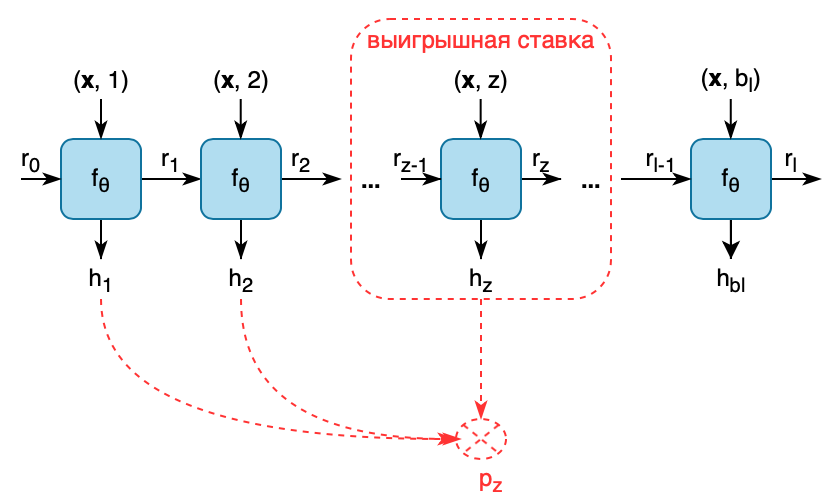
\includegraphics{nn_rnn_layer.png}
\end{figure}

В третей части подсказываем условную вероятность для каждого блока. 
Для этого используется рекуррентная LSTM сеть. 
Так как все вероятности должны быть в интервале $(0;1)$, то на выходе из этого слоя, используется монотонно возрастающая функция сигмоида.

На выходе мы получается условные вероятности проигрыша для каждой ставки.
С помощью формул (~\ref{eq:nnW}, ~\ref{eq:nnS}, ~\ref{eq:nnP}) можно посчитать вероятности выигрыша, проигрыша и плотности распределения рыночной цены.

\subsection{Обучение нейронной сети}

Для обучения используется две функции ошибки. 
Первая основана на плотности распределения и ее основная цель минимизировать ANLP для всех выигрышных случаев (обозначим их как $D_{win}$).

\begin{equation}
    \begin{split}
        L_1 & = - \log \prod_{(x^i, z^i) \in D_{win}} p_l^i = - \log \prod_{(x^i, z^i) \in D_{win}} h_{l_i}^i \prod_{l: l < l^i} (1 - h_l^i) \\
        & = - \sum_{(x^i, z^i) \in D_{win}} \left[\log h_{l_i}^i + \sum_{l: l < l^i} \log (1 - h_l^i)\right]
    \end{split}
\end{equation}

Где $l^i$ – номер интервала, в который входит рыночная цена $z^i \in V_{l^i}$ для $i$-ого примера.

Вторая ошибка основывается на функции распределения и разбита на две части. 
В случае выигрыша аукциона необходимо <<занижать>> вероятность выигрыша в интервале $[0, z]$, и <<завышаем>> в интервале $[z, \infty)$.

\begin{equation}
    \begin{split}
        L_{win} & = - \log \prod_{(x^i, z^i) \in D_{win}} Pr(b^i > z \mid x^i; \Theta) \\
        & = - \log \prod_{(x^i, z^i) \in D_{win}} W(b^i \mid x^i; \Theta) \\
        & = - \sum_{(x^i, z^i) \in D_{win}} \log \left[1 - \prod_{l: l < l^i} (1 - h_l^i)\right]
    \end{split}
\end{equation}

В случае проигрыша рыночная цена не известна, поэтому можно только <<занизить>> вероятность выигрыша в интервале $[0, b]$.

\begin{equation}
    \begin{split}
        L_{lose} & = - \log \prod_{(x^i, z^i) \in D_{lose}} Pr(b^i \leq z \mid x^i; \Theta) \\
        & = - \log \prod_{(x^i, z^i) \in D_{lose}} S(b^i \mid x^i; \Theta) \\
        & = - \sum_{(x^i, z^i) \in D_{lose}} \sum_{l: l \leq l^i} \log (1 - h_l^i)
    \end{split}
\end{equation}

Чтобы использовать обе ошибки вместе введем простую формулу $w$, которая зависит только от ставки и рыночной цены в аукционе.

\begin{equation}
    w = \begin{cases}
        1, & \mbox{если } b > z \\ 0, & \mbox{если } b \leq z
    \end{cases}
\end{equation}

Тогда вторую функцию ошибки $L_2$ можно расписать как сумму $L_{win}$ и $L_{lose}$.

\begin{equation}
    \begin{split}
        L_2 & = L_{win} + L_{lose} \\
        & = - log \prod_{(x^i, b^i) \in D_{win}} Pr(b^i > z \mid x^i; \Theta) - log \prod_{(x^i, b^i) \in D_{lose}} Pr(z \geq b^i \mid x^i; \Theta) \\
        & = - \log \prod_{(x^i, z^i) \in D} {[W(b^i \mid x^i; \Theta)]}^{w^i} \cdot {\left[1 - W(b^i \mid x^i; \Theta)\right]}^{1 - w^i} \\
        & = - \sum_{(x^i, b^i) \in D} \left[w^i \log W(b^i \mid x^i; \Theta) + (1 - w^i) log (1 - W(b^i \mid x^i; \Theta)) \right]
    \end{split}
\end{equation}

Для обучения модели будет использоваться комбинация двух формул.

\begin{equation}
    \argmin_{\Theta} \alpha L_1 + \beta L_2
\end{equation}

Где $\alpha$ и $\beta$ гиперпараметры, которые контролируют величину градиента для стабилизации обучения модели.

\section{Подходы к улучшению показателей нейронной сети}

\subsection{Механизм внимания}

Один из первых подходов для улучшения модели было применение механизма внимания.

Будем применять механизм для скрытого состояния рекуррентного слоя для создания вектора контекста. 
После применим этот вектор для каждого блока ставки. 
С помощью этого, наша сеть получит доступ к необходимой информации 
о том каким параметрам уделять больше внимания при предсказании распределения, в каждом скрытом состоянии.

\begin{figure}[h]
    \caption{Иллюстрация нейронной сети с механизмом внимания}
    \centering
    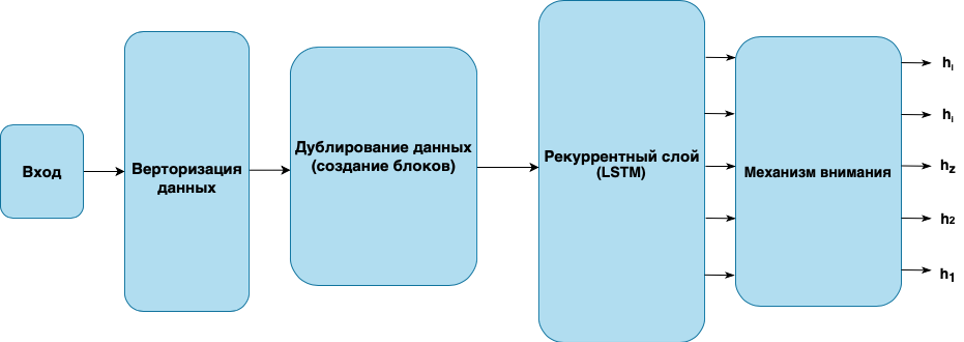
\includegraphics{nn_attention.png}
\end{figure}

\subsection{Pruning нейронной сети}

Основная идея в облегчении модели нейронной сети, путем удаления некоторого количества нейронов и связей, при этом с сохранением качества модели. 
Элементы сети, которые оказывают небольшое влияние на ошибку аппроксимации, будут исключаться без значительного ухудшения качества модели.

\subsection{Улучшение loss-функции}

Хотим добавить дополнительную функцию ошибки для регуляризации всего процесса обучения. 
По аналогии с решениями из Survival analysis, где используется третья функция ошибся для регуляции 
при различных замерах показателей при наблюдении за пациентом.

\subsection{Использование альтернативного решения из Survival analysis}

\chapterconclusion

В данном разделе были описаны существующие решения поставленной задачи, 
решение с помощью нейронных сетей, которое взято за baseline, 
также было описано реализованное решение и подходы к него улучшению.

\chapter{Практическое исследование}

\section{Описание датасета}

Для обучения и тестирования использовался открытый датасет компании iPinYou.
Этот датасет публичный, что дает возможность сравнивать результаты алгоритмов из других статей. 

В датасете содержатся информация об аукционах для 9 различных рекламных объявлений, 
каждые из которых находятся в разных сферах. 
Данные разделены на две части: датасет для обучения (train) и для тестирования (test).

\begin{table}
    \label{table:ipinyou}
    \centering
    \footnotesize
    \begin{tabular}{c c c c c}
        \hline
        № объявления & Выигрышные (train) & Проигрышные (train) & Выигрышные (test) & Проигрышные (test) \\ [0.5ex]
        \hline
        1458 & 997247 & 2085809 & 119397 & 495241 \\
        2259 & 296657 & 538899 & 99626 & 317571 \\
        2261 & 221454 & 466163 & 100477 & 243385 \\
        2821 & 142697 & 1179864 & 86136 & 575828 \\
        2997 & 43803 & 268634 & 26944 & 129119 \\
        3358 & 278637 & 1463467 & 36373 & 264555 \\
        3386 & 683319 & 2164483 & 136128 & 409293 \\
        3427 & 501868 & 2091897 & 153121 & 383674 \\
        3476 & 644951 & 1325409 & 78896 & 444952 \\ [1ex]
        \hline
    \end{tabular}
    \caption{Описание датасета iPinYou}
\end{table}

\section{Метрики качества модели}

Для метрики качества используются показатели ANLP и ROC-кривая. 
Первая – это функция ошибки, которая используется при обучении, 
вторая – метрика для классификаторов, которая позволяет оценить точность и качество модели.

\section{Сравнение с актуальным решением}

\begin{table}[!h]
    \caption{Сравнение показателей по ANLP}
    \centering
    \begin{tabular}{c c c c c}
        \hline
        № объявления & KM & STM & baseline & текущее решение \\ [0.5ex]
        \hline
        1458 & 10.532 & 4.761 & \infty & \infty \\
        2259 & 14.671 & 5.471 & \infty & \infty \\
        2261 & 14.665 & 4.818 & \infty & \infty \\
        2821 & 19.582 & 5.572 & \infty & \infty \\
        2997 & 16.203 & 5.083 & 2.2743 & 0.5439 \\
        3358 & 19.253 & 5.539 & \infty & \infty \\
        3386 & 15.973 & 5.228 & \infty & \infty \\
        3427 & 16.902 & 5.321 & \infty & \infty \\
        3476 & 10.507 & 4.537 & 1.4686 & 1.4222 \\ [1ex]
        \hline
    \end{tabular}
\end{table}

\begin{table}
    \caption{Сравнение показателей по C-index (ROC-AUC)}
    \centering
    \begin{tabular}{c c c c c}
        \hline
        № объявления & KM & STM & baseline & текущее решение \\ [0.5ex]
        \hline
        1458 & 0.698 & 0.764 & 0.904 & \infty \\
        2259 & 0.685 & 0.768 & 0.876 & \infty \\
        2261 & 0.666 & 0.812 & 0.929 & \infty \\
        2821 & 0.677 & 0.790 & 0.881 & \infty \\
        2997 & 0.734 & 0.835 & 0.919 & 0.9236 \\
        3358 & 0.704 & 0.811 & 0.944 & \infty \\
        3386 & 0.716 & 0.849 & 0.923 & \infty \\
        3427 & 0.724 & 0.798 & 0.901 & \infty \\
        3476 & 0.692 & 0.830 & 0.922 & 0.924 \\ [1ex]
    \end{tabular}
\end{table}

\chapterconclusion

В этой главе был описан датасет, на котором происходит обучение и тестирования моделей.
Введены метрики для проверки качества модели. 
Опубликованы первые результаты работы алгоритма.

%% Макрос для заключения. Совместим со старым стилевиком.
\startconclusionpage

В данном разделе размещается заключение.

\printmainbibliography

%% После этой команды chapter будет генерировать приложения, нумерованные русскими буквами.
%% \startappendices из старого стилевика будет делать то же самое
\appendix

\end{document}
